\documentclass[11pt]{amsart}
\usepackage[utf8]{inputenc}
\usepackage[T1]{fontenc}
\usepackage{amsmath}
\usepackage{verbatim}
\usepackage{hyperref}
\usepackage{float}

\usepackage{tikz}

\usetikzlibrary{arrows}

\voffset=-20mm
\textheight=245mm
\textwidth=155mm 
\oddsidemargin=5mm
\evensidemargin=5mm

\title{Derivation of backpropagation}

\begin{document}

\maketitle

\section{Notation}

Suppose we have a neural network built for a binary classification task (see Fig.~\ref{fig:nn} for example). For binary classification we are solving an optimization task:
$$F(b) = - \dfrac{1}{N} \displaystyle\sum_{k = 1}^N \bigl[ y_k \ln p_k + (1 - y_k) \ln (1 - p_k) \bigr] \rightarrow \min_b,$$
where $N$ --- batch size, $y_k$ --- true label of the $k$-th object, $p_k = a_L(x_k)$ --- output of the network on the $k$-th object, $b$ --- set of neural network parameters.



\begin{figure}[H]
    \centering

    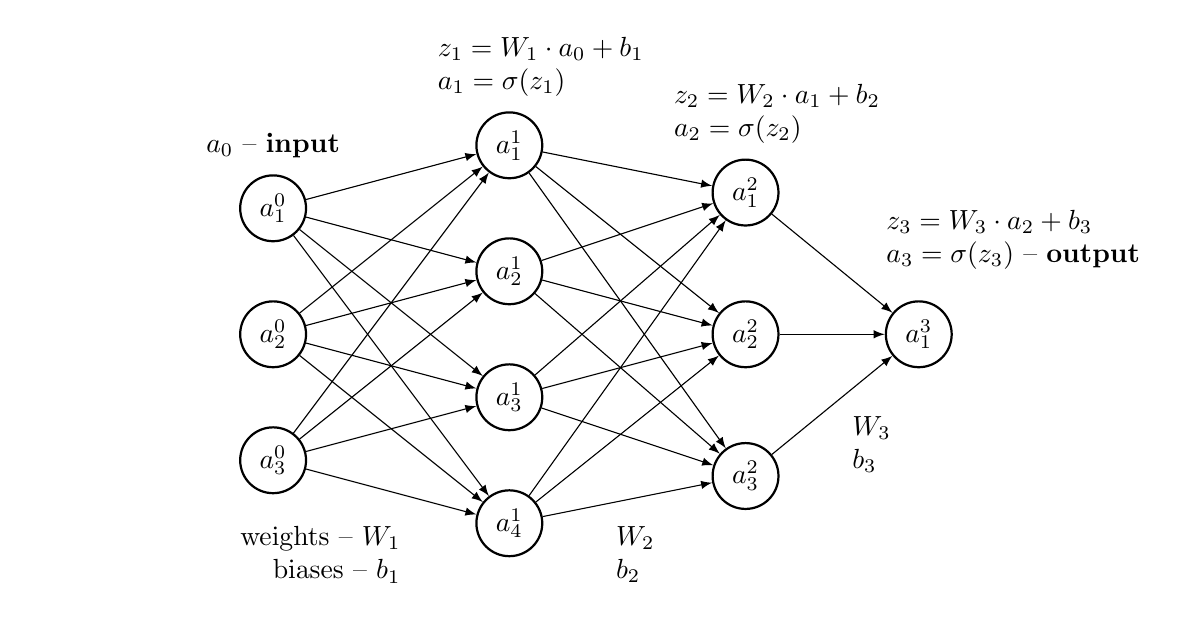
\begin{tikzpicture}[scale=0.2]
        \node (a10) at (0, 8) [draw, circle, thick] {$a_1^0$};
        \node (a20) at (0, 0) [draw, circle, thick] {$a_2^0$};
        \node (a30) at (0, -8) [draw, circle, thick] {$a_3^0$};

        \node (a11) at (15, 12) [draw, circle, thick] {$a_1^1$};
        \node (a21) at (15, 4) [draw, circle, thick] {$a_2^1$};
        \node (a31) at (15, -4) [draw, circle, thick] {$a_3^1$};
        \node (a41) at (15, -12) [draw, circle, thick] {$a_4^1$};

        \node (a12) at (30, 9) [draw, circle, thick] {$a_1^2$};
        \node (a22) at (30, 0) [draw, circle, thick] {$a_2^2$};
        \node (a32) at (30, -9) [draw, circle, thick] {$a_3^2$};

        \node (a13) at (41, 0) [draw, circle, thick] {$a_1^3$};

        \foreach \a in {a10, a20, a30}
            \foreach \b in {a11, a21, a31, a41}
                {\draw [-latex] (\a) -- (\b);}

        \foreach \a in {a11, a21, a31, a41}
            \foreach \b in {a12, a22, a32}
                {\draw [-latex] (\a) -- (\b);}

        \foreach \a in {a12, a22, a32}
            \foreach \b in {a13}
                {\draw [-latex] (\a) -- (\b);}

        \node at (0, 12) {$a_0$ -- {\bf input}};
        \node at (17, 17) [align=left] {$z_1 = W_1 \cdot a_0 + b_1$ \\  $a_1 = \sigma(z_1)$};
        \node at (32, 14) [align=left] {$z_2 = W_2 \cdot a_1 + b_2$ \\  $a_2 = \sigma(z_2)$};
        \node at (47, 6) [align=left] {$z_3 = W_3 \cdot a_2 + b_3$ \\  $a_3 = \sigma(z_3)$ -- {\bf output}};

        \node at (3, -14) [align=right] {weights -- $W_1$ \\ biases -- $b_1$};
        \node at (23, -14) [align=left] {$W_2$ \\ $b_2$};
        \node at (38, -7) [align=left] {$W_3$ \\ $b_3$};

        \node at (-15, 0) {};
    \end{tikzpicture}

    \caption{A feed-forward neural network architecture}
    \label{fig:nn}
\end{figure}



We are going to use the following notation:
\begin{itemize}
    \item $0$ --- input layer, $L$ --- output layer,
    \item $n_l$ --- $l$-th layer size,
    \item $a_l = (a_i^l)_{(n_l \times 1)}$ --- $l$-th layer output, $a_0$ --- input,
    \item $W_l = (w_{ij}^l)_{(n_i \times n_{i - 1})}$ --- weights, $b_l = (b_i^l)_{(n_l \times 1)}$ --- biasses connecting $l$-th layer with ($l - 1$)-th layer,
    \item $z_l = W_l \cdot a_{l - 1} + b_l$ --- $l$-th layer before activation,
    \item $\sigma(x) = \dfrac{1}{1 + e^{-x}}$ --- sigmoid function, $\sigma'(x) = \sigma(x) (1 - \sigma(x))$,
    \item <<$\ast$>> --- element-size multiplication, <<$\cdot$>> -- matrix multiplication.
\end{itemize}



\bigskip

\section{Gradient derivation}

In order to calculate the gradient vector $\nabla F$, we need to calculate each partial derivative~$\dfrac{\partial F}{\partial w_{ij}^l}$ and $\dfrac{\partial F}{\partial b_i^l}$.

We start with the derivative
$$\dfrac{\partial F}{\partial z_L} = \dfrac{\partial F}{\partial a_L} \dfrac{\partial a_L}{\partial z_L}$$
Strictly speaking, this is a matrix, nevertheless the non-diagonal derivatives (i.e. $\dfrac{\partial a_i^L}{\partial z_j^L}$ for $i \neq j$) are zeros, thus, in fact this is a vector of size $n_L$.

First, suppose the batch size is $N = 1$. In this case
$$F = - y \ln a_L - (1 - y) \ln (1 - a_L)$$
and
$$\dfrac{\partial F}{\partial a_L} = - \dfrac{y}{a_L} + \dfrac{1 - y}{1 - a_L}
    = \dfrac{- y (1 - a_L) + (1 - y) a_L}{a_L (1 - a_L)}
    = \dfrac{a_L - y}{a_L (1 - a_L)}$$
For the second factor $\dfrac{\partial a_L}{\partial z_L}$, since $a_L = \sigma (z_L)$, we have
$$\dfrac{\partial a_L}{\partial z_L} = \sigma(z_L) (1 - \sigma (z_L)) = a_L (1 - a_L)$$
Putting it all together, we have
$$\dfrac{\partial F}{\partial z_L} = a_L - y$$

We are going to get back to this layer later, but for now let us establish how to derive $\dfrac{\partial L}{\partial z_l}$ using $\dfrac{\partial L}{\partial z_{l + 1}}$ for $l < L$. We have
$$\dfrac{\partial L}{\partial z_l} = \dfrac{\partial L}{\partial z_{l + 1}} \dfrac{\partial z_{l + 1}}{\partial a_l} \dfrac{\partial a_l}{\partial z_l},$$
since $z_{l + 1} = W_{l + 1} \cdot a_l + b_{l + 1}$. By induction, we can assume that the first factor $\dfrac{\partial L}{\partial z_{l + 1}}$ has already been calculated on the previous step and is a vector of size $n_{l + 1}$. The second factor~$\dfrac{\partial z_{l + 1}}{\partial a_l}$ is a matrix of size $n_{i + 1} \times n_l$. In fact, this is exactly the matrix $W_{l + 1}$. Finally, the last factor $\dfrac{\partial a_l}{\partial z_l}$ is simply the sigmoid derivative. Thus,
$$\dfrac{\partial F}{\partial z_l} = W_{l + 1}^\top \cdot \dfrac{\partial F}{\partial z_{l + 1}} \ast \bigl( \sigma(z_l) \ast (1 - \sigma(z_l)) \bigr),$$
where $\sigma(z_l)$ is element-wise.

In this fashion we can calculate each partial derivative of $F$ over $z_l$. Since each $z_l$ is linear with respect to $W_l$ and $b_l$, we have:
$$\dfrac{\partial z_l}{\partial W_l} = a_{l - 1}^\top, \:\: \dfrac{\partial z_l}{\partial b_l} = 1$$

The final formulas:
$$\dfrac{\partial F}{\partial W_l} = \dfrac{\partial F}{\partial z_L} \cdot a_{l - 1}^\top, \:\: \dfrac{\partial F}{\partial b_l} = \dfrac{\partial F}{\partial z_l}$$

Finally, the gradient vector $\nabla F$ consists of all the partial derivatives over $W_l$ and $b_l$, but we do not actually need to put them all into a vector, since we only need their values.

\end{document}
